% !TeX root = ../../thesis.tex
\chapter{Implementation of finite difference method} \label{ch_numerical_implementation}
\section*{General information}
The 2D system was discretized into a rectangular equidistant grid and rearranged into a single column vector as indicated in figure~\ref{fig_sketch_2D_to_column}. The differential operators were represented by finite-difference matrices left-multiplying the column vectors standing for field variables present on the grid. The finite-difference matrices are block matrices, where each block is a square matrix acting on a single column in the rearranged system.\\
Let the system be a matrix with $n$ rows and $m$ columns. All blocks are matrices with dimensions $n\times n$ and they are ordered in $m\times m$ grid giving rise to an $mn\times mn$ sparse finite-difference matrix .\\
The finite-difference matrix can perform linear combination of arbitrary points in the system in each grid point. It takes various form depending on the boundary conditions. However, it is always a toeplitz block matrix.

Second-order accurate centered finite-difference scheme in space and first-order in time (i.e. the Euler method) were used.

In the following sections, the symbol $\mathbb{O}$ stands for $n\times n$ block matrix of zeros and $\mathbb{I}$ for $n\times n$ identity matrix (i.e. matrix with ones in the diagonal and zeros otherwise). The finite difference method is abbreviated as FD in the following. In the finite-difference matrices below, some elements may be highlighted in red. These are the elements, which are involved in the boundary conditions.


\begin{figure}[h]
	\centering
	% \vspace{3cm}
	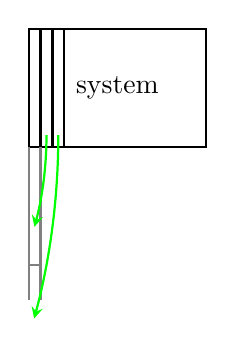
\begin{tikzpicture}[scale=1.5]
		% box & columns
		\draw[thick] (0,0) -- (1.5,0) -- (1.5,1) -- (0,1) -- cycle; 
		\draw[thick] (0.1,0) -- (0.1,1);
		\draw[thick] (0.2,0) -- (0.2,1);
		\draw[thick] (0.3,0) -- (0.3,1);
		% reordered system to vector
		\draw[thick,color=gray] (0,0) -- (0,-1);
		\draw[thick,color=gray] (0.1,-1) -- (0,-1);
		\draw[thick,color=gray] (0.1,-1) -- (0.1,0);
		\draw[thick,color=gray] (0,-1.3) -- (0,-1);
		\draw[thick,color=gray] (0.1,-1.3) -- (0.1,-1);
		% arrows
		\draw[thick,color=green,-stealth]  (0.15,0.1) arc (0:-15:3cm);
		\draw[thick,color=green,-stealth]  (0.25,0.1) arc (0:-15:6cm);
		% label
		\draw (0.75,0.5) node {system};
	\end{tikzpicture} 
	\caption{Rearrangement of the matrix representing the system before application of the discrete deferential operators.}
	\label{fig_sketch_2D_to_column}
\end{figure}

\section*{Ghost nodes in Neumann boundary condition}

\subsection*{Zero Neumann BCs}
Neumann boundary conditions were implemented using ghost nodes. Ghost nodes are hypothetical nodes adjacent to the boundary nodes, in which the values can be specified using the given boundary condition. In order to have the derivatives in the boundary nodes second-order-accurate, centered difference can be used using the known values at ghost nodes. In the case $\nabla\eta\cdot\bm{n}=0$ we can write at the left boundary edge (i.e. $x=0$), where $(i,j)=(0,j)$
\begin{equation} \label{eq_neumanBC_ghost_pts_value}
	\begin{split}
		\frac{\partial \eta}{\partial x}=0 \quad \mathrm{at}\,x=0 \quad &\Rightarrow\quad \forall j\in m+1 \; (\Delta_x\eta)_{0j} = \frac{\eta_{1j}-\eta_{-1j}}{h} = 0 \quad \implies\quad \eta_{1j}=\eta_{-1j} \\
		\frac{\partial \eta}{\partial y}=0 \quad \mathrm{at}\,x=0 \quad &\Rightarrow\quad \forall i\in n+1 \; (\Delta_y\eta)_{0j}= \frac{\eta_{ij+1}-\eta_{ij-1}}{h}  
	\end{split}
\end{equation}

The first equation provides the value at the ghost node. In order to have the centered difference in the respective direction zero at the boundary, apparently the value must be equal to the value in the neighbour on the opposite side.

\subsection*{General Neumann BCs}
The boundary condition defining the inclination angle $\theta$ at the boundary is $\nabla\eta\cdot\bm{n}=|\nabla\eta|\cos(\theta)$. This expression implies at the left boundary $(i,j)=(0,j)$  that $\frac{\partial \eta}{\partial x}=|\nabla\eta|\cos(\theta)$ and $\frac{\partial \eta}{\partial y}=|\nabla\eta|\sin(\theta)$. By replacing the partial derivatives $\frac{\partial}{\partial x},\frac{\partial}{\partial y}$ with finite differences $\Delta_x, \Delta_y$ the values in ghost node $(-1,j)$ can be expressed as 
\begin{align}
	\forall j\in m+1 \quad (\Delta_x \eta)_{0j} = \frac{\eta_{1j}-\eta_{-1j}}{2h} = |\nabla\eta|_{0,j}\cos(\theta) \\
		\quad\implies\quad \eta_{-1j}=\eta_{1j} - 2h|\nabla\eta|_{0j}\cos(\theta) \,.
\end{align}
At the right boundary $(i,j)=(n,j)$ the ghost nodes $(n+1,j)$ are
\begin{align}
	\forall j\in m+1 \quad (\Delta_x \eta)_{nj} = \frac{\eta_{n+1j}-\eta_{n-1j}}{2h} = |\nabla\eta|_{nj}\cos(\theta) \\
		\quad \implies\quad \eta_{n+1j}=\eta_{n-1j} + 2h|\nabla\eta|_{nj}\cos(\theta) \,.
\end{align}
And at the bottom and top, respectively, using the same principles we obtain
\begin{align}
	\forall i\in n+1 \quad  \eta_{i,-1}&=\eta_{i,1} - 2h|\nabla\eta|_{i,0}\cos(\theta) \\
	\forall i\in n+1 \quad  \eta_{i,m+1}&=\eta_{i,m-1} + 2h|\nabla\eta|_{i,m}\cos(\theta) 
	\,.
\end{align}
Important observation is that the general Neumann BC indeed reduces to the zero condition for $\theta=90$\textdegree and that the values at the ghost nodes are always derived from the neighbour on the opposite side. 

\section*{First-order derivatives in FD}
The centered finite difference was used with stencil  \begin{tabular}{|c|c|c|}
	\hline -1&0&1  \\\hline
\end{tabular} 
for x-direction derivative and
\begin{tabular}{|c|}
	\hline1  \\\hline
	0 \\\hline
	-1 \\\hline
\end{tabular} 
for y-direction derivative. 
\subsection*{Periodic boundary conditions}
For the y-direction derivative the FD matrix is
\begin{equation} \label{eq_FDmatrix_der1_y}
	\frac{\partial }{\partial y} \approx \Delta_y= \frac{1}{2h}\left(\begin{array}{cccccc}
		\mathbb{Y} & \mathbb{O} & \mathbb{O}& \dots&\mathbb{O} &\mathbb{O}\\
		\mathbb{O}&\mathbb{Y} &  \mathbb{O}& \dots&\mathbb{O}&\mathbb{O}\\
		\mathbb{O}&\mathbb{O}&\mathbb{Y} & \dots &  \mathbb{O}&\mathbb{O}\\
		\vdots&\vdots&\vdots&\ddots &\vdots&\vdots\\
		\mathbb{O}&\mathbb{O}&\mathbb{O}&\dots &\mathbb{Y} & \mathbb{O} \\
		\mathbb{O}&\mathbb{O}&\mathbb{O}&\dots &\mathbb{O}&\mathbb{Y}
	\end{array}\right)
\end{equation}
with
\begin{equation}
	\mathbb{Y} = \left(\begin{array}{cccccccc}
		0 & 1 & 0&  0 & \dots & 0 & 0 & \red -1 \bk\\
		-1 & 0 &  1& 0 & \dots& 0 & 0 & 0\\
		0 &-1&0 & 1 & \dots & 0 & 0 & 0\\
		\vdots&\vdots&\vdots&\ddots &\vdots&\vdots&\vdots&\vdots\\
		0 & 0 & 0 &0 &  \dots & -1 & 0 & 1 \\
		\red 1 \bk & 0 & 0 &0 &  \dots & 0 &-1 &0
	\end{array}\right)
\end{equation}
In the x-direction, the finite difference matrix is
\begin{equation}
	\frac{\partial }{\partial x} \approx \Delta_x = \frac{1}{2h}
	\left(\begin{array}{cccccccc}
		\mathbb{O} & \mathbb{I} & \mathbb{O}& \mathbb{O}&\dots &\mathbb{O} &  \mathbb{O} & \red -\mathbb{I} \bk \\
		-\mathbb{I}&\mathbb{O} &  \mathbb{I}& \mathbb{O}&\dots&\mathbb{O}&  \mathbb{O}&\mathbb{O}\\
		\mathbb{O}& -\mathbb{I}&\mathbb{O} & \mathbb{I}& \dots & \mathbb{O}&  \mathbb{O}&  \mathbb{O}\\
		\vdots&\vdots&\vdots&\ddots &\vdots&\vdots&\vdots&\vdots\\
		\mathbb{O}&\mathbb{O}&\mathbb{O}&\mathbb{O}&\dots & -\mathbb{I}&  \mathbb{O} & \mathbb{I} \\
		\red\mathbb{I} \bk&\mathbb{O}&\mathbb{O}&\mathbb{O}&\dots &\mathbb{O}& -\mathbb{I} &\mathbb{O}
	\end{array}\right) \,.
\end{equation}


\subsection*{Neumann boundary conditions}
The FD matrices are equal in both cases of the zero and general NBC, but in the case of the gerneral NBC the following vector must be added at the left and right boundary $|\nabla\eta|\left[\begin{array}{c}
	\cos(\theta)  \\
	\sin(\theta) 
\end{array}\right]$ and the following one at the bottom and top boundary  $|\nabla\eta|\left[\begin{array}{c}
	-\sin(\theta)  \\
	\cos(\theta)
\end{array}\right]$.

For the y-direction the FD matrix is the same as for the periodic boundary conditions in the block structure (equation \ref{eq_FDmatrix_der1_y}), and the block matrix $\mathbb{Y}$ is only modified in its first and last row as
\begin{equation}
	\mathbb{Y} = \left(\begin{array}{cccccccc}
		0 & 0 & 0&  0 & \dots & 0 & 0 & 0 \\
		-1 & 0 &  1& 0 & \dots& 0 & 0 & 0\\
		0 &-1&0 & 1 & \dots & 0 & 0 & 0\\
		\vdots&\vdots&\vdots&\ddots &\vdots&\vdots&\vdots&\vdots\\
		0 & 0 & 0 &0 &  \dots & -1 & 0 & 1 \\
		0 & 0 & 0 &0 &  \dots & 0 &0  &0
	\end{array}\right)
\end{equation}
For the x-direction with Neoumann boundary conditions
\begin{equation}
	\frac{\partial }{\partial x} \approx \Delta_x = \frac{1}{2h}
	\left(\begin{array}{cccccccc}
		\mathbb{O} & \mathbb{O} & \mathbb{O}& \mathbb{O}&\dots &\mathbb{O} &  \mathbb{O} &  \mathbb{O}  \\
		-\mathbb{I}&\mathbb{O} &  \mathbb{I}& \mathbb{O}&\dots&\mathbb{O}&  \mathbb{O}&\mathbb{O}\\
		\mathbb{O}& -\mathbb{I}&\mathbb{O} & \mathbb{I}& \dots & \mathbb{O}&  \mathbb{O}&  \mathbb{O}\\
		\vdots&\vdots&\vdots&\ddots &\vdots&\vdots&\vdots&\vdots\\
		\mathbb{O}&\mathbb{O}&\mathbb{O}&\mathbb{O}&\dots & -\mathbb{I}&  \mathbb{O} & \mathbb{I} \\
		\mathbb{O} &\mathbb{O} &\mathbb{O}&\mathbb{O}&\dots &\mathbb{O}& \mathbb{O} &\mathbb{O}
	\end{array}\right)
\end{equation}

\subsection*{Mixed boundary conditions}
In 2D system there are only two options when combining periodic and Neumann BCs: the periodic boundary is either parallel to x or y axis. The periodic boundary must always lay opposite to another periodic boundary. In a system with mixed boundaries the finite difference matrices in the x and y direction are combined from the above options so that the BCs are met at the corresponding boundary. 

\section*{Laplacian in 2D}
5-point stencil 
\begin{tabular}{c|c|c}
	0&1&0  \\\hline
	1&-4&1 \\\hline
	0&1&0
\end{tabular} 
approximates 2D laplacian $\nabla^2 u = u_{xx}+u_{yy}$ on an bi-equidistant grid with spacing $h$ in a grid point $(i,j)$ as
\begin{equation}
	(\nabla^2u)_{ij}^{\mathrm{5p}} = u_{ij,xx} + u_{ij,yy} = \frac{1}{h^2}(-4u_{ij} + u_{i-1j}+ u_{i+1j}+ u_{ij-1}+ u_{ij+1}) + \mathcal{O}(h^4)
\end{equation}

9-point stencil (denoted 9p8)
\begin{tabular}{c|c|c}
	1&1&1  \\\hline
	1&-8&1 \\\hline
	1&1&1
\end{tabular} 
is expressed in a grid point $(i,j)$ as
\begin{equation}
	\begin{split}
		(\nabla^2u)_{ij}^{\mathrm{9p8}} &=  \frac{1}{3h^2}(-8u_{ij} + u_{i-1j}+ u_{i+1j}+ u_{ij-1}+ u_{ij+1} +\\
		&\quad+ u_{i+1j+1}+u_{i-1j-1}+u_{i-1j+1}+u_{i+1j-1}) + \mathcal{O}(h^4)
	\end{split}
\end{equation}

9-point stencil (denoted 9p20)
\begin{tabular}{c|c|c}
	1&4&1  \\\hline
	4&-20&4 \\\hline
	1&4&1
\end{tabular} 
is expressed in a grid point $(i,j)$ as
\begin{equation}
	\begin{split}
		(\nabla^2u)_{ij}^{\mathrm{9p20}} &=  \frac{1}{6h^2}[-20u_{ij} + 4(u_{i-1j}+ u_{i+1j}+ u_{ij-1}+ u_{ij+1}) +\\
		&\quad+ u_{i+1j+1}+u_{i-1j-1}+u_{i-1j+1}+u_{i+1j-1}] + \mathcal{O}(h^4)
	\end{split}
\end{equation}

The above formulas are derived from Taylor expansions of the values of function $u$ at the points adjacent to $(i,j)$ assuming the small displacement $h$ in both x and y direction.

The above formulas are represented by matrix, which carries the weighted summation of the function values for each point similarly to the first-order derivatives. Below, the matrices are shown in detail depending on the BCs. 

\subsection*{Periodic boundary conditions}
For 5p stencil the blocks are unit matrix $\mathbb{I}$, zero matrix $\mathbb{O}$ and the following matrix $\mathbb{D}^{\mathrm{5p}}$ (the red elements are the top-bottom periodic condition) 
\begin{equation}
	\begin{split}
		\mathbb{D}^{\mathrm{5p}}_P &= \left(\begin{array}{ccccccccc}
			-4 & 1 & 0&0& \dots&0&0 &\red 1\bk\\
			1&-4&1&0&\dots&0&0& 0\\
			0&1&-4&1 &\dots&0&0&0\\
			\vdots&\vdots&\vdots&\vdots&\ddots &\vdots&\vdots&\vdots\\
			0&0&0&0&\dots &1&-4&1 \\
			\red 1\bk&0&0&0&\dots &0&1&-4
		\end{array}\right).
	\end{split}
\end{equation}
and the finite-difference matrix $\mathbb{L}^{\mathrm{5p}}$ is ordered as follows (red elements are the left-right periodic boundary condition)
\begin{equation}
	\mathbb{L}^{\mathrm{5p}}_P = \frac{1}{h^2}\left(\begin{array}{cccccccccc}
		\mathbb{D}^{\mathrm{5p}}_P & \mathbb{I} & \mathbb{O}&\mathbb{O}& \dots&\mathbb{O}&\mathbb{O} &\red \mathbb{I}\bk\\
		\mathbb{I}&\mathbb{D}^{\mathrm{5p}}_P & \mathbb{I} & \mathbb{O}& \dots&\mathbb{O}&\mathbb{O}&\mathbb{O}\\
		\mathbb{O}&\mathbb{I}&\mathbb{D}^{\mathrm{5p}}_P & \mathbb{I} &  \dots&\mathbb{O}&\mathbb{O}&\mathbb{O}\\
		\vdots&\vdots&\vdots&\vdots&\ddots &\vdots&\vdots&\vdots\\
		\mathbb{O}&\mathbb{O}&\mathbb{O}&\mathbb{O}&\dots &\mathbb{I}&\mathbb{D}^{\mathrm{5p}}_P & \mathbb{I} \\
		\red \mathbb{I}\bk&\mathbb{O}&\mathbb{O}&\mathbb{O}&\dots &\mathbb{O}&\mathbb{I}&\mathbb{D}^{\mathrm{5p}}_P
	\end{array}\right)
\end{equation}

For 9p20 stencil the blocks are a Toeplitz matrix $\mathbb{D}^{\mathrm{9p20}}_P$, a Toeplitz matrix $\mathbb{A}$ and a zero matrix $\mathbb{O}$. These are defined
\begin{align}
	\mathbb{D}^{\mathrm{9p20}}_P &= \left(\begin{array}{ccccccccc}
		-20 & 4 & 0&0& \dots&0&0 &\red 4\bk\\
		4&-20&4&0&\dots&0&0& 0\\
		0&4&-20&4 &\dots&0&0&0\\
		\vdots&\vdots&\vdots&\vdots&\ddots &\vdots&\vdots&\vdots\\
		0&0&0&0&\dots &4&-20&4 \\
		\red 4\bk&0&0&0&\dots &0&4&-20
	\end{array}\right) \\
	%
	\mathbb{A} &= \left(\begin{array}{ccccccccc}
		4 & 1 & 0&0& \dots&0&0 &\red 1\bk\\
		1&4&1&0&\dots&0&0& 0\\
		0&1&4&1 &\dots&0&0&0\\
		\vdots&\vdots&\vdots&\vdots&\ddots &\vdots&\vdots&\vdots\\
		0&0&0&0&\dots &1&4&1 \\
		\red 1\bk&0&0&0&\dots &0&1&4
	\end{array}\right)
\end{align}
and arranged 
\begin{equation}
	\mathbb{L}^{\mathrm{9p20}}_P = \frac{1}{6h^2}\left(\begin{array}{cccccccccc}
		\mathbb{D}^\mathrm{9p20}_P & \mathbb{A} & \mathbb{O}&\mathbb{O}& \dots&\mathbb{O}&\mathbb{O} &\red \mathbb{A}\bk\\
		\mathbb{A}&\mathbb{D}^\mathrm{9p20}_P & \mathbb{A} & \mathbb{O}& \dots&\mathbb{O}&\mathbb{O}&\mathbb{O}\\
		\mathbb{O}&\mathbb{A}&\mathbb{D}^\mathrm{9p20}_P & \mathbb{A} &  \dots&\mathbb{O}&\mathbb{O}&\mathbb{O}\\
		\vdots&\vdots&\vdots&\vdots&\ddots &\vdots&\vdots&\vdots\\
		\mathbb{O}&\mathbb{O}&\mathbb{O}&\mathbb{O}&\dots &\mathbb{A}&\mathbb{D}^\mathrm{9p20}_P & \mathbb{A} \\
		\red \mathbb{A}\bk&\mathbb{O}&\mathbb{O}&\mathbb{O}&\dots &\mathbb{O}&\mathbb{A}&\mathbb{D}^\mathrm{9p20}_P
	\end{array}\right)
\end{equation}

\subsection*{Neuman boundary conditions}
For both zero and general NBCs the FD matrices are equal. Because the value at ghost nodes is either equal or derived from value of neighbour on the opposite side, the laplacian stencil behaves at the Neumann boundary as in Figure~\ref{fig_laplacian_NBC}.
\begin{figure}
	\centering
	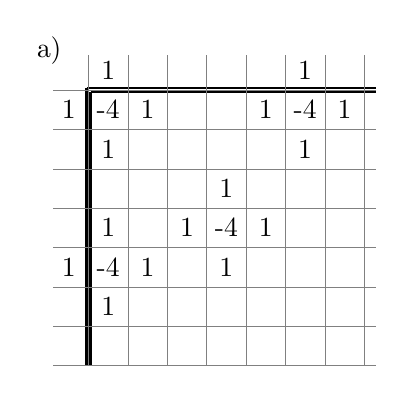
\begin{tikzpicture}[scale=0.5]
		\draw (-1,8) node {a)};
		% box & columns
		\draw[thick] (0.05,6.95) -- (7.3,6.95); 
		\draw[thick] (0.05,6.95) -- (0.05,0); 
		\draw[thick] (-0.05,7.05) -- (7.3,7.05); 
		\draw[thick] (-0.05,7.05) -- (-0.05,0); 
		
		\draw[step=1cm,very thin,color=gray] (7.3,7.9) grid  (-0.9,0);
		% corner
		\draw (0.5,6.5) node {-4};
		\draw (1.5,6.5) node {1};
		\draw (-0.5,6.5) node {1};
		\draw (0.5,7.5) node {1};
		\draw (0.5,5.5) node {1};
		% bulk
		\draw (3.5,3.5) node {-4};
		\draw (3.5,2.5) node {1};
		\draw (3.5,4.5) node {1};
		\draw (2.5,3.5) node {1};
		\draw (4.5,3.5) node {1};
		% top
		\draw (5.5,6.5) node {-4};
		\draw (4.5,6.5) node {1};
		\draw (6.5,6.5) node {1};
		\draw (5.5,7.5) node {1};
		\draw (5.5,5.5) node {1};
		% left
		\draw (0.5,2.5) node {-4};
		\draw (0.5,3.5) node {1};
		\draw (0.5,1.5) node {1};
		\draw (1.5,2.5) node {1};
		\draw (-0.5,2.5) node {1};
	\end{tikzpicture} 
	%
	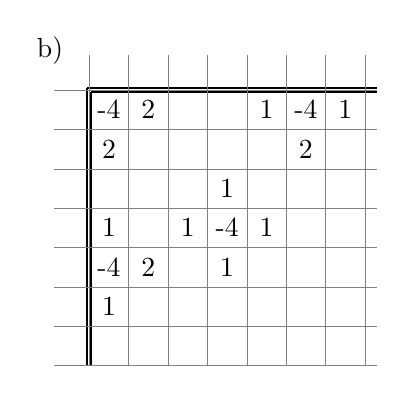
\begin{tikzpicture}[scale=0.5]
		\draw (-1,8) node {b)};
		% box & columns
		\draw[thick] (0.05,6.95) -- (7.3,6.95); 
		\draw[thick] (0.05,6.95) -- (0.05,0); 
		\draw[thick] (-0.05,7.05) -- (7.3,7.05); 
		\draw[thick] (-0.05,7.05) -- (-0.05,0); 
		%
		\draw[step=1cm,very thin,color=gray] (7.3,7.9) grid  (-0.9,0);
		% corner
		\draw (0.5,6.5) node {-4};
		\draw (1.5,6.5) node {2};
		\draw (0.5,5.5) node {2};
		% bulk
		\draw (3.5,3.5) node {-4};
		\draw (3.5,2.5) node {1};
		\draw (3.5,4.5) node {1};
		\draw (2.5,3.5) node {1};
		\draw (4.5,3.5) node {1};
		% top
		\draw (5.5,6.5) node {-4};
		\draw (4.5,6.5) node {1};
		\draw (6.5,6.5) node {1};
		\draw (5.5,5.5) node {2};
		% left
		\draw (0.5,2.5) node {-4};
		\draw (0.5,3.5) node {1};
		\draw (0.5,1.5) node {1};
		\draw (1.5,2.5) node {2};
	\end{tikzpicture} 
	\caption[Effect of Neuman BC on the 5pt laplacian stencil on the boundary points]{Effect of Neuman BC on the 5pt laplacian stencil on the boundary points. Ghost points are outside the simulation domain but they can be accounted for thanks to knowing their value from equation~\ref{eq_neumanBC_ghost_pts_value}.}
	\label{fig_laplacian_NBC}
\end{figure}

The 5p stencil finite-differnce matrix $\mathbb{L}^{\mathrm{5p}}_N$ with Neuman BC is composed of 4 different blocks: tridiagonal $\mathbb{D}^{\mathrm{5p}}_{N}$, unit matrix $\mathbb{I}$, $2\mathbb{I}$ and zero matrix $\mathbb{O}$. These are:
\begin{align}
	\mathbb{D}^{\mathrm{5p}}_{N} &= \left(\begin{array}{ccccccccc}
		-4 & \red 2\bk & 0&0& \dots&0&0 &0\\
		1&-4&1&0&\dots&0&0& 0\\
		0&1&-4&1 &\dots&0&0&0\\
		\vdots&\vdots&\vdots&\vdots&\ddots &\vdots&\vdots&\vdots\\
		0&0&0&0&\dots &1&-4&1 \\
		0&0&0&0&\dots &0&\red 2\bk&4
	\end{array}\right) \\
\end{align}
and are ordered as follows
\begin{equation}
	\mathbb{L}^{\mathrm{5p}}_N = \frac{1}{h^2}\left(\begin{array}{cccccccccc}
		\mathbb{D}^{\mathrm{5p}}_{N} & \red 2\mathbb{I} \bk& \mathbb{O}&\mathbb{O}& \dots&\mathbb{O}&\mathbb{O} & \mathbb{O}\\
		\mathbb{I}&\mathbb{D}^{\mathrm{5p}}_{N} & \mathbb{I} & \mathbb{O}& \dots&\mathbb{O}&\mathbb{O}&\mathbb{O}\\
		\mathbb{O}&\mathbb{I}&\mathbb{D}^{\mathrm{5p}}_{N} & \mathbb{I} &  \dots&\mathbb{O}&\mathbb{O}&\mathbb{O}\\
		\vdots&\vdots&\vdots&\vdots&\ddots &\vdots&\vdots&\vdots\\
		\mathbb{O}&\mathbb{O}&\mathbb{O}&\mathbb{O}&\dots &\mathbb{I}&\mathbb{D}^{\mathrm{5p}}_{N} & \mathbb{I} \\
		\mathbb{O}&\mathbb{O}&\mathbb{O}&\mathbb{O}&\dots &\mathbb{O}&\red 2\mathbb{I}\bk&\mathbb{D}^{\mathrm{5p}}_{N}
	\end{array}\right)
\end{equation}    

In case of general NBC in 5-point stencil there must always be added or subtracted the term $2h|\nabla\eta|_{ij}\cos(\theta) $, where $(i,j)$ are the boundary points. At the left and bottom boundary it is subtracted, at the right and top it is added.

The 9p20 stencil finite-differnce matrix $\mathbb{L}^{\mathrm{9p20}}_N$ with Neuman BC is composed of 4 differnt blocks: tridiagonal $\mathbb{D}^{\mathrm{9p20}}_N$, tridiagonal $\mathbb{B}$, $2\mathbb{B}$ and zero matrix $\mathbb{O}$. These are
\begin{align}
	\mathbb{D}^{\mathrm{9p20}}_N &= \left(\begin{array}{ccccccccc}
		-20 & \red 8\bk & 0&0& \dots&0&0 &0\\
		4&-20&4&0&\dots&0&0& 0\\
		0&4&-20&4 &\dots&0&0&0\\
		\vdots&\vdots&\vdots&\vdots&\ddots &\vdots&\vdots&\vdots\\
		0&0&0&0&\dots &4&-20&4 \\
		0&0&0&0&\dots &0&\red 8\bk&-20
	\end{array}\right) \\
	%
	\mathbb{B} &= \left(\begin{array}{ccccccccc}
		4 & \red 2\bk & 0&0& \dots&0&0 &0\\
		1&4&1&0&\dots&0&0& 0\\
		0&1&4&1 &\dots&0&0&0\\
		\vdots&\vdots&\vdots&\vdots&\ddots &\vdots&\vdots&\vdots\\
		0&0&0&0&\dots &1&4&1 \\
		0&0&0&0&\dots &0&\red 2\bk&4
	\end{array}\right)
\end{align}
and are ordered as follows
\begin{equation}
	\mathbb{L}^{\mathrm{9p20}}_N = \frac{1}{6h^2}\left(\begin{array}{cccccccccc}
		\mathbb{D}^\mathrm{9p20}_N & \red 2\mathbb{B} \bk& \mathbb{O}&\mathbb{O}& \dots&\mathbb{O}&\mathbb{O} & \mathbb{O}\\
		\mathbb{B}&\mathbb{D}^\mathrm{9p20}_N & \mathbb{B} & \mathbb{O}& \dots&\mathbb{O}&\mathbb{O}&\mathbb{O}\\
		\mathbb{O}&\mathbb{B}&\mathbb{D}^\mathrm{9p20}_N & \mathbb{B} &  \dots&\mathbb{O}&\mathbb{O}&\mathbb{O}\\
		\vdots&\vdots&\vdots&\vdots&\ddots &\vdots&\vdots&\vdots\\
		\mathbb{O}&\mathbb{O}&\mathbb{O}&\mathbb{O}&\dots &\mathbb{B}&\mathbb{D}^\mathrm{9p20}_N & \mathbb{B} \\
		\mathbb{O}&\mathbb{O}&\mathbb{O}&\mathbb{O}&\dots &\mathbb{O}&\red 2\mathbb{B}\bk&\mathbb{D}^\mathrm{9p20}_N
	\end{array}\right)
\end{equation}    
In case of general NBC in 9-point stencil the term $2h|\nabla\eta|_{ij}\cos(\theta) $ must be added or subtracted (depending on the boundary) correspondingly to the stencil, e.g. at the left boundary
\begin{equation}
	\frac{1}{6h^2}\begin{array}{c|c|c}
		1&4&1  \\ \hline
		4&-20&4 \\ \hline
		1&4&1
	\end{array} \rightarrow  
	\frac{1}{6h^2} \left[\begin{array}{c|c|c}
		0&4&2  \\ \hline
		0&-20&8 \\ \hline
		0&4&2
	\end{array} - 2h\cos(\theta)(|\nabla\eta|_{0,j+1} + |\nabla\eta|_{0,j-1} + 4|\nabla\eta|_{0,j}) \right]
\end{equation}
or e.g. at the top boundary
\begin{equation}
	\frac{1}{6h^2}\begin{array}{c|c|c}
		1&4&1  \\ \hline
		4&-20&4 \\ \hline
		1&4&1
	\end{array} \rightarrow  
	\frac{1}{6h^2} \left[\begin{array}{c|c|c}
		0&0&0  \\ \hline
		4&-20&4 \\ \hline
		2&8&2
	\end{array} + 2h\cos(\theta)(|\nabla\eta|_{i+1,M} + |\nabla\eta|_{i-1,M} + 4|\nabla\eta|_{i,M}) \right]
\end{equation}

\subsection*{Mixed boundary conditions}
Imagine the system with BCs as indicated in figure~\ref{fig_scheme_mixedBC}.
\begin{figure}
	\centering
	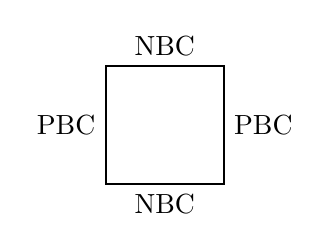
\begin{tikzpicture}[scale=0.5]
		\draw[thick] (0,0) -- node[midway,left] {PBC} (0,3) -- node[midway,above] {NBC}  (3,3) -- node[midway, right] {PBC} (3,0) -- node[midway,below] {NBC}  cycle; 
	\end{tikzpicture} 
	\caption[Layout of the mixed boundaries]{Layout of the mixed boundaries. NBC and PBC stand for Neumann and periodic boundary conditions, respectively.}
	\label{fig_scheme_mixedBC}
\end{figure}
The action of the finite difference matrix in the y-direction is given by the structure of the individual block matrices and the x-direction by the arrangement of the blocks in the large matrix.\\
Specifically, with the periodic BCs present in the x-direction, the structure of the large matrix is as with periodic BCs only the diagonal block matrix. Showing on the example of the 5pt laplacian approximation with mixed BCs as in the figure~\ref{fig_scheme_mixedBC}
\begin{equation}
	\mathbb{L}^{\mathrm{5p}}_{PN} = \frac{1}{h^2}\left(\begin{array}{cccccccccc}
		\mathbb{D}^{\mathrm{5p}}_N & \mathbb{I} & \mathbb{O}&\mathbb{O}& \dots&\mathbb{O}&\mathbb{O} &\red \mathbb{I}\bk\\
		\mathbb{I}&\mathbb{D}^{\mathrm{5p}}_N & \mathbb{I} & \mathbb{O}& \dots&\mathbb{O}&\mathbb{O}&\mathbb{O}\\
		\mathbb{O}&\mathbb{I}&\mathbb{D}^{\mathrm{5p}}_N & \mathbb{I} &  \dots&\mathbb{O}&\mathbb{O}&\mathbb{O}\\
		\vdots&\vdots&\vdots&\vdots&\ddots &\vdots&\vdots&\vdots\\
		\mathbb{O}&\mathbb{O}&\mathbb{O}&\mathbb{O}&\dots &\mathbb{I}&\mathbb{D}^{\mathrm{5p}}_N & \mathbb{I} \\
		\red \mathbb{I}\bk&\mathbb{O}&\mathbb{O}&\mathbb{O}&\dots &\mathbb{O}&\mathbb{I}&\mathbb{D}^{\mathrm{5p}}_N
	\end{array}\right)
\end{equation}

In the 9p20 scheme the finite difference matrix is
\begin{equation}
	\mathbb{L}^{\mathrm{9p20}}_{PN} = \frac{1}{6h^2}\left(\begin{array}{cccccccccc}
		\mathbb{D}^\mathrm{9p20}_N & \mathbb{A} & \mathbb{O}&\mathbb{O}& \dots&\mathbb{O}&\mathbb{O} &\red \mathbb{A}\bk\\
		\mathbb{A}&\mathbb{D}^\mathrm{9p20}_N & \mathbb{A} & \mathbb{O}& \dots&\mathbb{O}&\mathbb{O}&\mathbb{O}\\
		\mathbb{O}&\mathbb{A}&\mathbb{D}^\mathrm{9p20}_N & \mathbb{A} &  \dots&\mathbb{O}&\mathbb{O}&\mathbb{O}\\
		\vdots&\vdots&\vdots&\vdots&\ddots &\vdots&\vdots&\vdots\\
		\mathbb{O}&\mathbb{O}&\mathbb{O}&\mathbb{O}&\dots &\mathbb{A}&\mathbb{D}^\mathrm{9p20}_N & \mathbb{A} \\
		\red \mathbb{A}\bk&\mathbb{O}&\mathbb{O}&\mathbb{O}&\dots &\mathbb{O}&\mathbb{A}&\mathbb{D}^\mathrm{9p20}_N
	\end{array}\right)
\end{equation}

\section*{Anisotropic driving force terms}
In phase field method, usually it is better to keep the interface away from the domain boundary as the boundary conditions often impose specific, non-physical behavior of the interface.  In the case of general NBC and the intended use for the energy assessment, the proximity of interface to the domain boundary is deliberate.\\
In the implementation of the inclination-dependent model, the anisotropic driving force terms are calculated from numeric derivatives of various fields. Care must be taken to each of the numerical derivative in order to assure the control over the interface inclination at the domain boundary. \\
When the interface inclination is fixed, the anisotropic driving force terms have fixed value (Dirichlet BC). Some of these fields are numerically differentiated again. However, their values at the ghost nodes are unknown (to be used in centered finite difference), hence one-sided FD scheme must be used at the boundaries. In order to keep second-order accuracy at the boundaries, the following backward $\begin{array}{|c|}
	\hline 1/2 \\ \hline -2 \\ \hline\hline 3/2 \\ \hline
\end{array}$ and forward $\begin{array}{|c|}
	\hline -3/2 \\ \hline\hline 2 \\ \hline -1/2 \\ \hline
\end{array}$ FD schemes were used at the bottom and top boundary, respectively.

For the x-direction derivative the FD matrix is
\begin{equation} \label{eq_FDmatrix_der1_y}
	\frac{\partial }{\partial x} \approx \Delta_x= \frac{1}{2h}\left(\begin{array}{cccccccc}
		\red -3\mathbb{I} & \red 4\mathbb{I} & \red-\mathbb{I}& \mathbb{O}& \dots&\mathbb{O} &\mathbb{O} &\mathbb{O}\\
		-\mathbb{I}&\mathbb{O} &  \mathbb{I}& \mathbb{O}&\dots&\mathbb{O}&  \mathbb{O}&\mathbb{O}\\
		\mathbb{O}& -\mathbb{I}&\mathbb{O} & \mathbb{I}& \dots & \mathbb{O}&  \mathbb{O}&  \mathbb{O}\\
		\vdots&\vdots&\vdots&\ddots &\vdots&\vdots&\vdots&\vdots\\
		\mathbb{O}&\mathbb{O}&\mathbb{O}&\mathbb{O}&\dots & -\mathbb{I}&  \mathbb{O} & \mathbb{I} \\
		\mathbb{O}&\mathbb{O}&\mathbb{O}&\dots & \mathbb{O}&\red\mathbb{I} &\red-4\mathbb{I}& \red3\mathbb{I}
	\end{array}\right) \,.
\end{equation}


For the y-direction derivative the FD matrix is
\begin{equation} \label{eq_FDmatrix_der1_y}
	\frac{\partial }{\partial y} \approx \Delta_y= \frac{1}{h}\left(\begin{array}{cccccc}
		\mathbb{Y} & \mathbb{O} & \mathbb{O}& \dots&\mathbb{O} &\mathbb{O}\\
		\mathbb{O}&\mathbb{Y} &  \mathbb{O}& \dots&\mathbb{O}&\mathbb{O}\\
		\mathbb{O}&\mathbb{O}&\mathbb{Y} & \dots &  \mathbb{O}&\mathbb{O}\\
		\vdots&\vdots&\vdots&\ddots &\vdots&\vdots\\
		\mathbb{O}&\mathbb{O}&\mathbb{O}&\dots &\mathbb{Y} & \mathbb{O} \\
		\mathbb{O}&\mathbb{O}&\mathbb{O}&\dots &\mathbb{O}&\mathbb{Y}
	\end{array}\right)
\end{equation}
with

\begin{equation}
	\mathbb{Y} = \left(\begin{array}{cccccccc}
		\red -3/2 &\red 2 &\red -1/2  &  0 & \dots & 0 & 0 &  0 \\
		-1 & 0 &  1& 0 & \dots& 0 & 0 & 0\\
		0 &-1&0 & 1 & \dots & 0 & 0 & 0\\
		\vdots&\vdots&\vdots&\ddots &\vdots&\vdots&\vdots&\vdots\\
		0 & 0 & 0 &0 &  \dots & -1 & 0 & 1 \\
		0 & 0 & 0 &0 &  \dots &\red 1/2 &\red-2 &\red 3/2 
	\end{array}\right)
\end{equation}








%%%%%%%%%%%%%%%%%%%%%%%%%%%%%%%%%%%%%%%%%%%%%%%%%%
% Keep the following \cleardoublepage at the end of this file, 
% otherwise \includeonly includes empty pages.
\cleardoublepage

% vim: tw=70 nocindent expandtab foldmethod=marker foldmarker={{{}{,}{}}}
